\begin{frame}{are lists enough?}
\begin{itemize}
    \item for correctness --- sure
    \vspace{.5cm}
    \item want to efficiently access items
        \begin{itemize}
        \item \myemph{better than linear time} to find something
        \end{itemize}
    \item want to \myemph{represent relationships} more naturally
\end{itemize}
\end{frame}

\begin{frame}{inter-item relationships in lists}
\begin{tikzpicture}
\tikzset{>=Latex}
\node[draw] (n1) { 1 };
\node[draw,right=1cm of n1] (n2) { 2 };
\node[draw,right=1cm of n2] (n3) { 3 };
\node[draw,right=1cm of n3] (n4) { 4 };
\node[draw,right=1cm of n4] (n5) { 5 };
\foreach \x/\y in {1/2,2/3,3/4,4/5} {
    \draw[ultra thick,<->] (n\x) -- (n\y);
}
\end{tikzpicture}
\begin{itemize}
\item List: \textit{nodes} related to \myemph{predecessor}/\myemph{successor}
\end{itemize}
\end{frame}

\begin{frame}{trees}
\begin{itemize}
    \item trees: allow representing more relationships
        \begin{itemize}
        \item (but not arbitrary relationships --- see graphs later in semester)
        \end{itemize}
    \item restriction: single path from \textit{root} to every node
        \begin{itemize}
        \item implies single path from every node to every other node (possibly through root)
        \end{itemize}
\end{itemize}
\end{frame}

\begin{frame}{natural trees: phylogenetic tree}
\vspace{-.25cm}
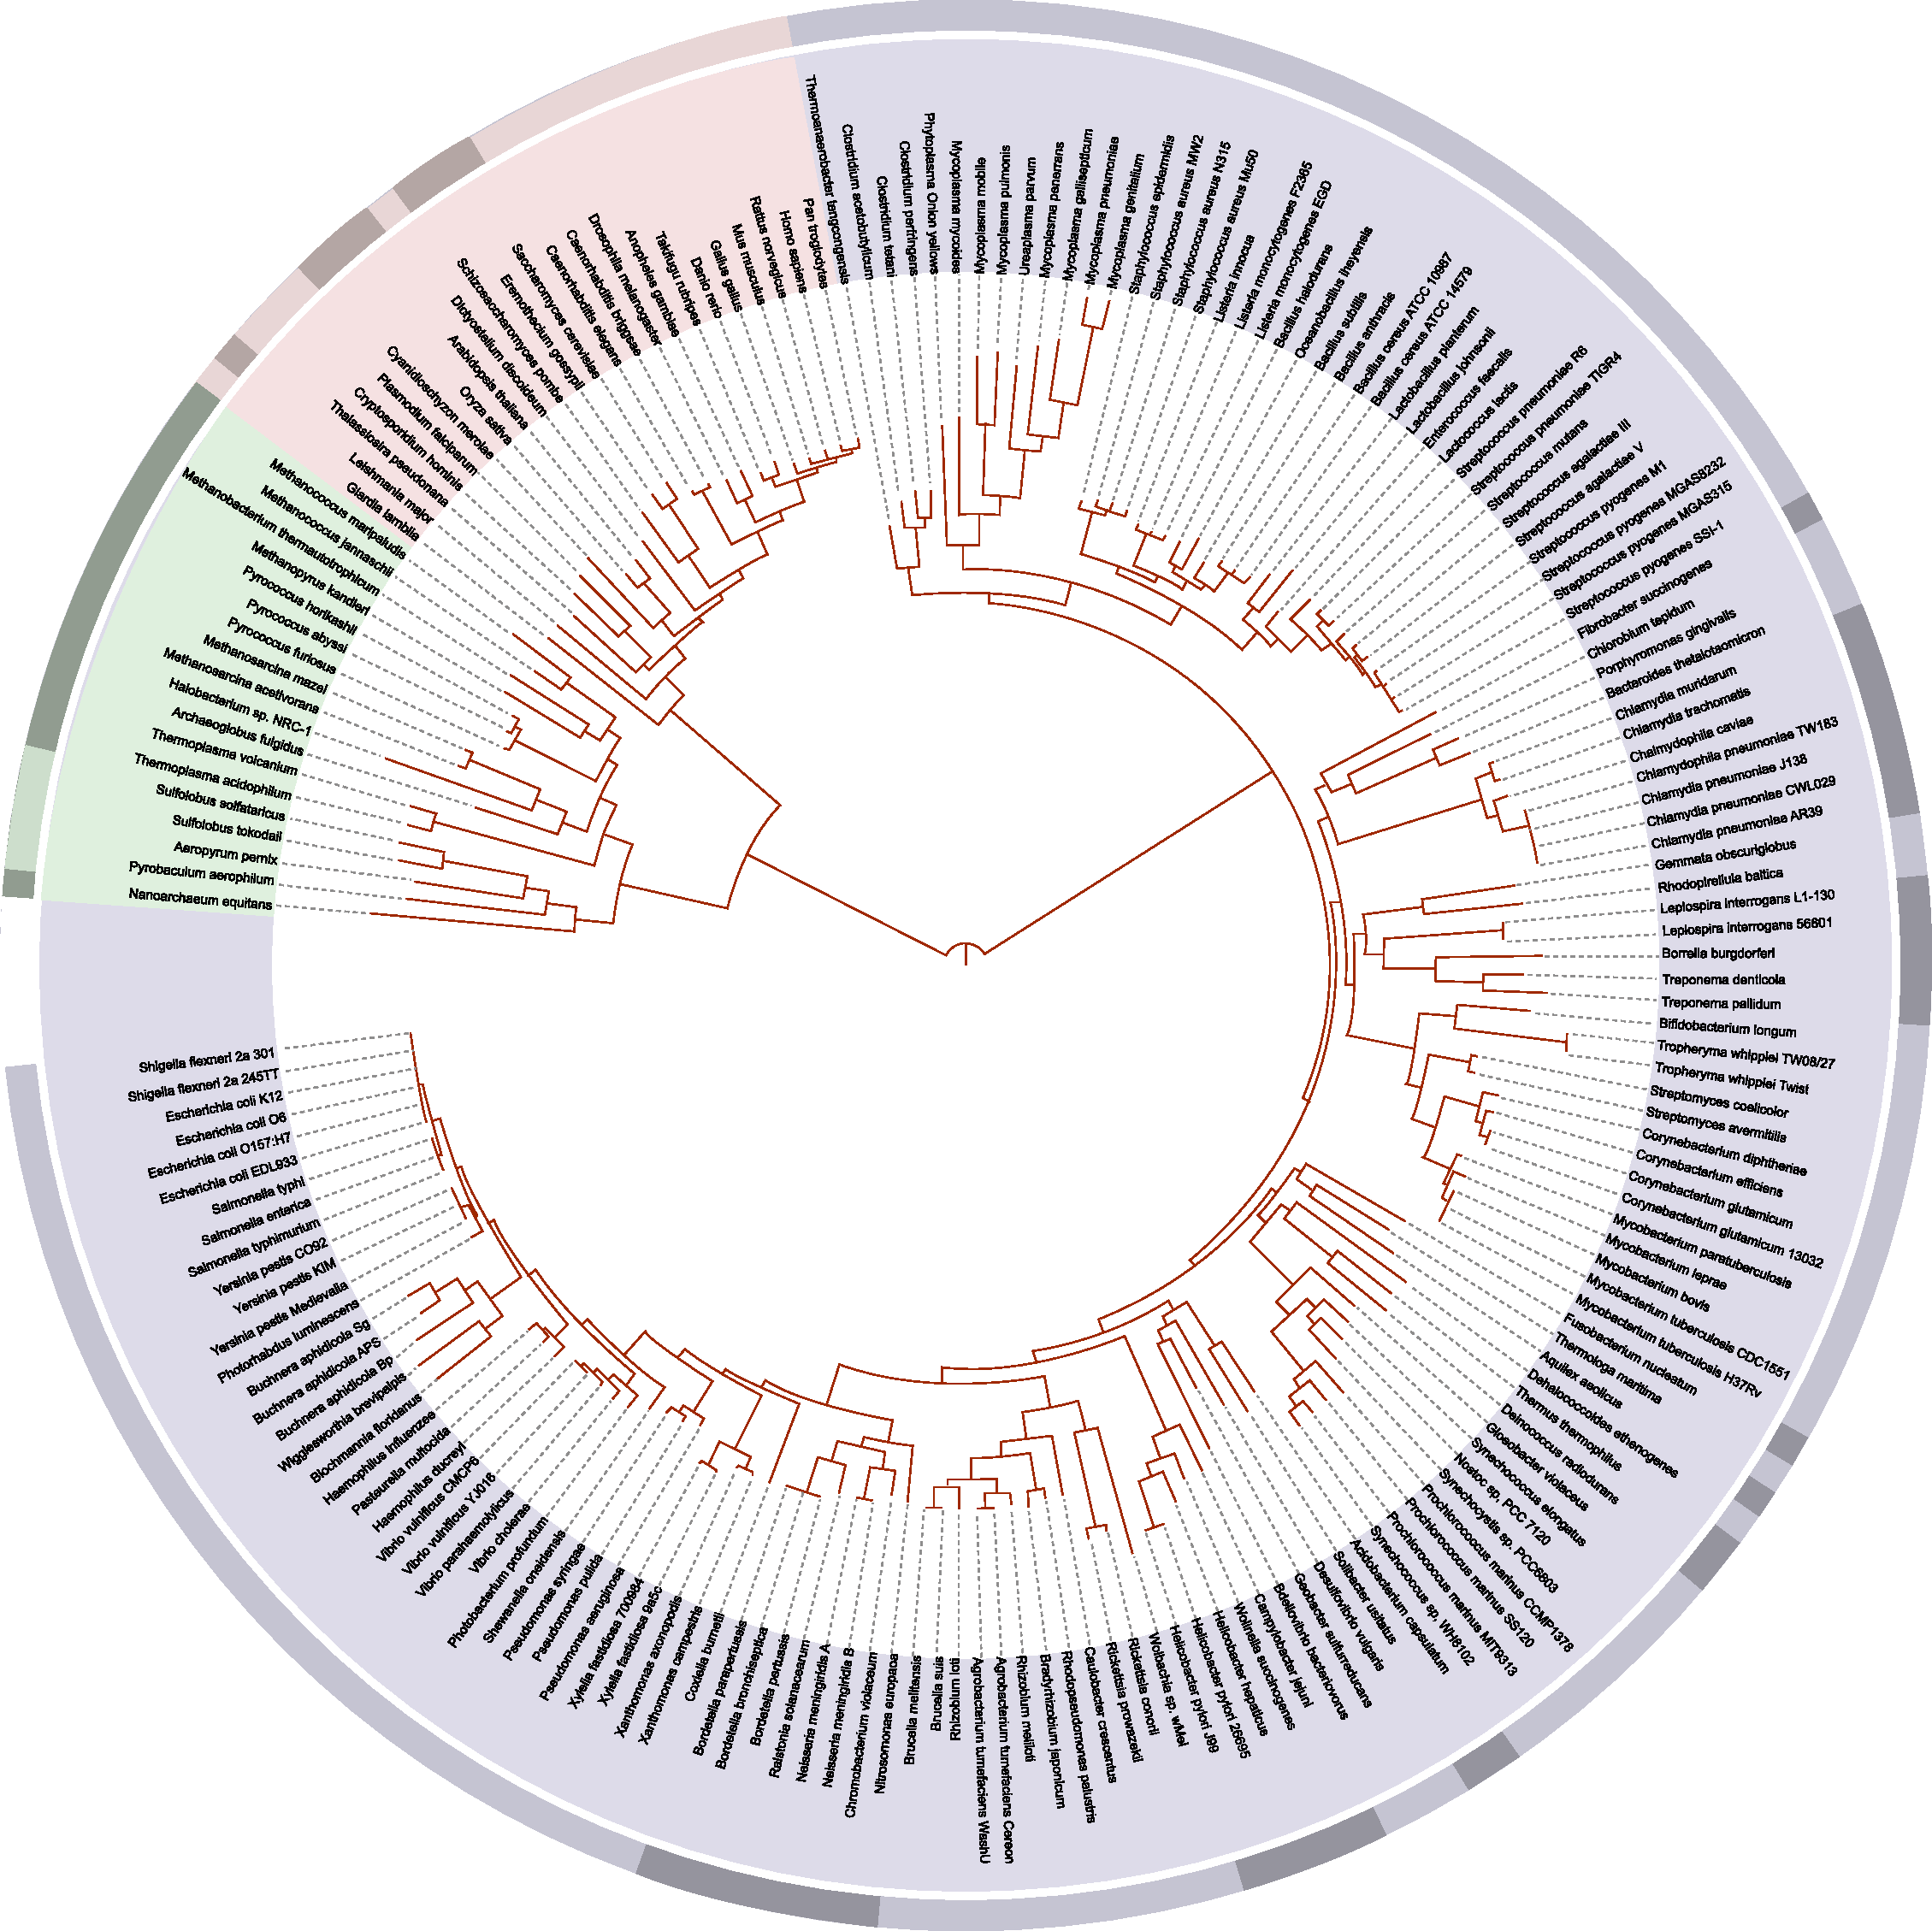
\includegraphics[height=0.9\textheight]{Tree_of_Life}
\imagecredit{image: Ivicia Letunic and Mariana Ruiz Villarreal, via the tool iTOL (Interative Tree of Life), via Wikipedia}
\end{frame}

\begin{frame}{natural trees: Indo-European languages}
\vspace{-.25cm}
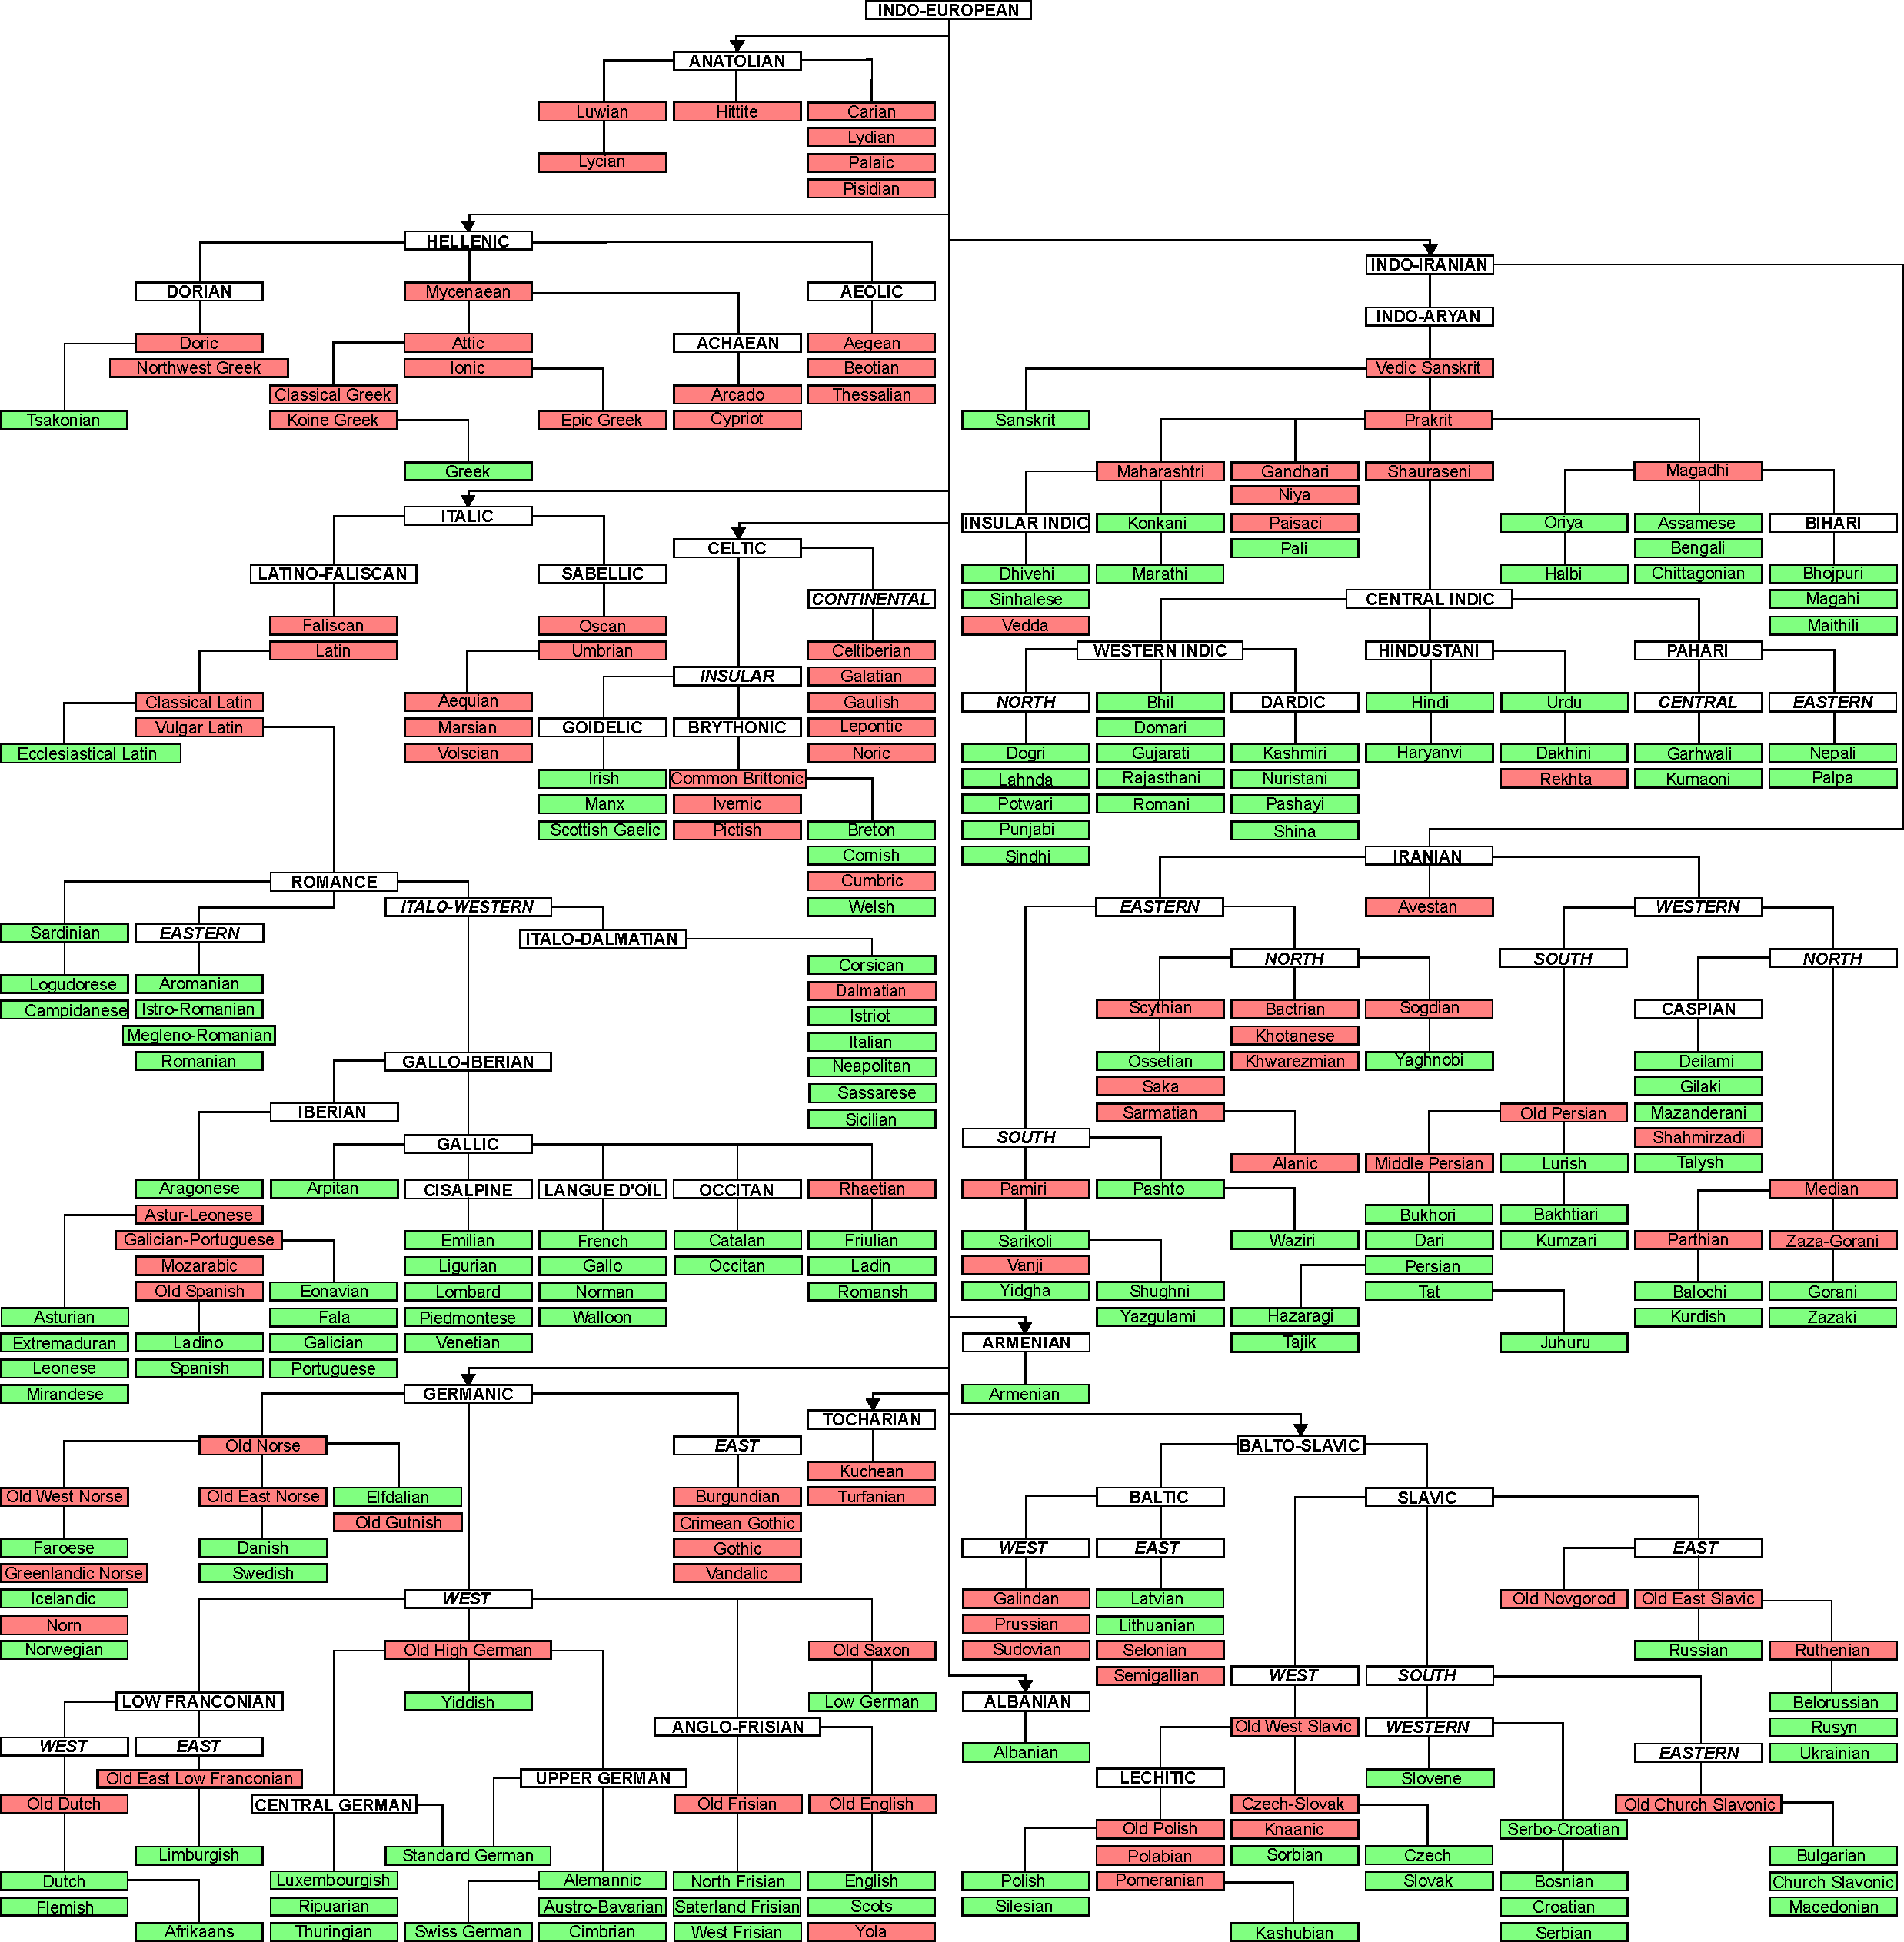
\includegraphics[height=0.9\textheight]{IndoEuropeanTree}
\imagecredit{image: via Wikipedia/Mandrak}
\end{frame}

\begin{frame}{list to tree}
\begin{tikzpicture}
\tikzset{>=Latex}
\begin{scope}[start chain=going right,every join/.style={->,very thick}]
\node[draw,thick,on chain] {predecessor};
\node[draw,thick,on chain,join] (elem) {element};
\node[draw,thick,on chain,join] {successor};
\end{scope}
\node[above=.5cm of elem] {\textit{list} --- up to 2 related nodes};

\node[draw,below=2cm of elem] (parent) {parent};
\node[draw,below=1cm of parent] (elem2) {element};
\node[draw,below=1cm of elem2,xshift=-2cm] (leftChild) {left child};
\node[draw,below=1cm of elem2,xshift=2cm] (rightChild) {left child};
\draw[->,very thick] (parent) -- (elem2);
\draw[->,very thick] (elem2) -- (leftChild);
\draw[->,very thick] (elem2) -- (rightChild);
\node[above=.5cm of parent] {\textit{binary tree} --- up to 3 related nodes (list is special-case)};
\end{tikzpicture}
\end{frame}

\begin{frame}{more general trees}
\begin{tikzpicture}
\tikzset{>=Latex}
\node[draw] (parent) {parent};
\node[draw,below=1cm of parent] (elem2) {element};
\node[draw,below=1cm of elem2,xshift=-4cm] (leftChild) {child 1};
\node[draw,below=1cm of elem2,xshift=0cm] (middleChild) {child 2};
\node[draw,below=1cm of elem2,xshift=5cm] (rightChild) {child $n$};
\node[font=\large,left=1.5cm of rightChild]{\ldots};
\draw[->,very thick] (parent) -- (elem2);
\draw[->,very thick] (elem2) -- (leftChild);
\draw[->,very thick] (elem2) -- (middleChild);
\draw[->,very thick] (elem2) -- (rightChild);
\node[above=.5cm of parent,align=left] {\textit{tree} --- any number of relationships (binary tree is special case) \\ \hspace{2cm}at most one parent};
\end{tikzpicture}
\end{frame}
